\section{"Ubersicht verschiedener Barcodesysteme}
Zur Zeit befinden sich viele verschiedene Barcodesysteme in Benutzung. Manche sind spezifisch für einen bestimmten Wirtschaftszweig, andere wiederum findet man so gut wie überall. Dieser Abschnitt soll die bekanntesten und verbreitetsten Systeme vorstellen. Dabei wird eine Grobeinteilung anhand der Anzahl der Dimensionen des Codes vorgenommen.

\subsection{Eindimensionale Barcodes}
Eindimensionale Barcodes codieren Daten entlang ihrer Länge (also links und rechts); nicht ihrer Höhe (also oben und unten). Würde man nun eine Linie durch einen eindimensionalen Barcode ziehen, findet man diese Dimension. Dieses Vorgehen nutzen die meisten der verwendeten Laserscanner. Dass eindimensionale Barcodes meist sehr groß abgedruckt sind hat einen einfachen Grund: Je größer der Code, desto einfacher findet ihn ein Scanner.

\subsubsection{Strichcode}
\begin{wrapfigure}[7]{r}{0.45\textwidth}
	\centering
	\vspace{-0.2cm}
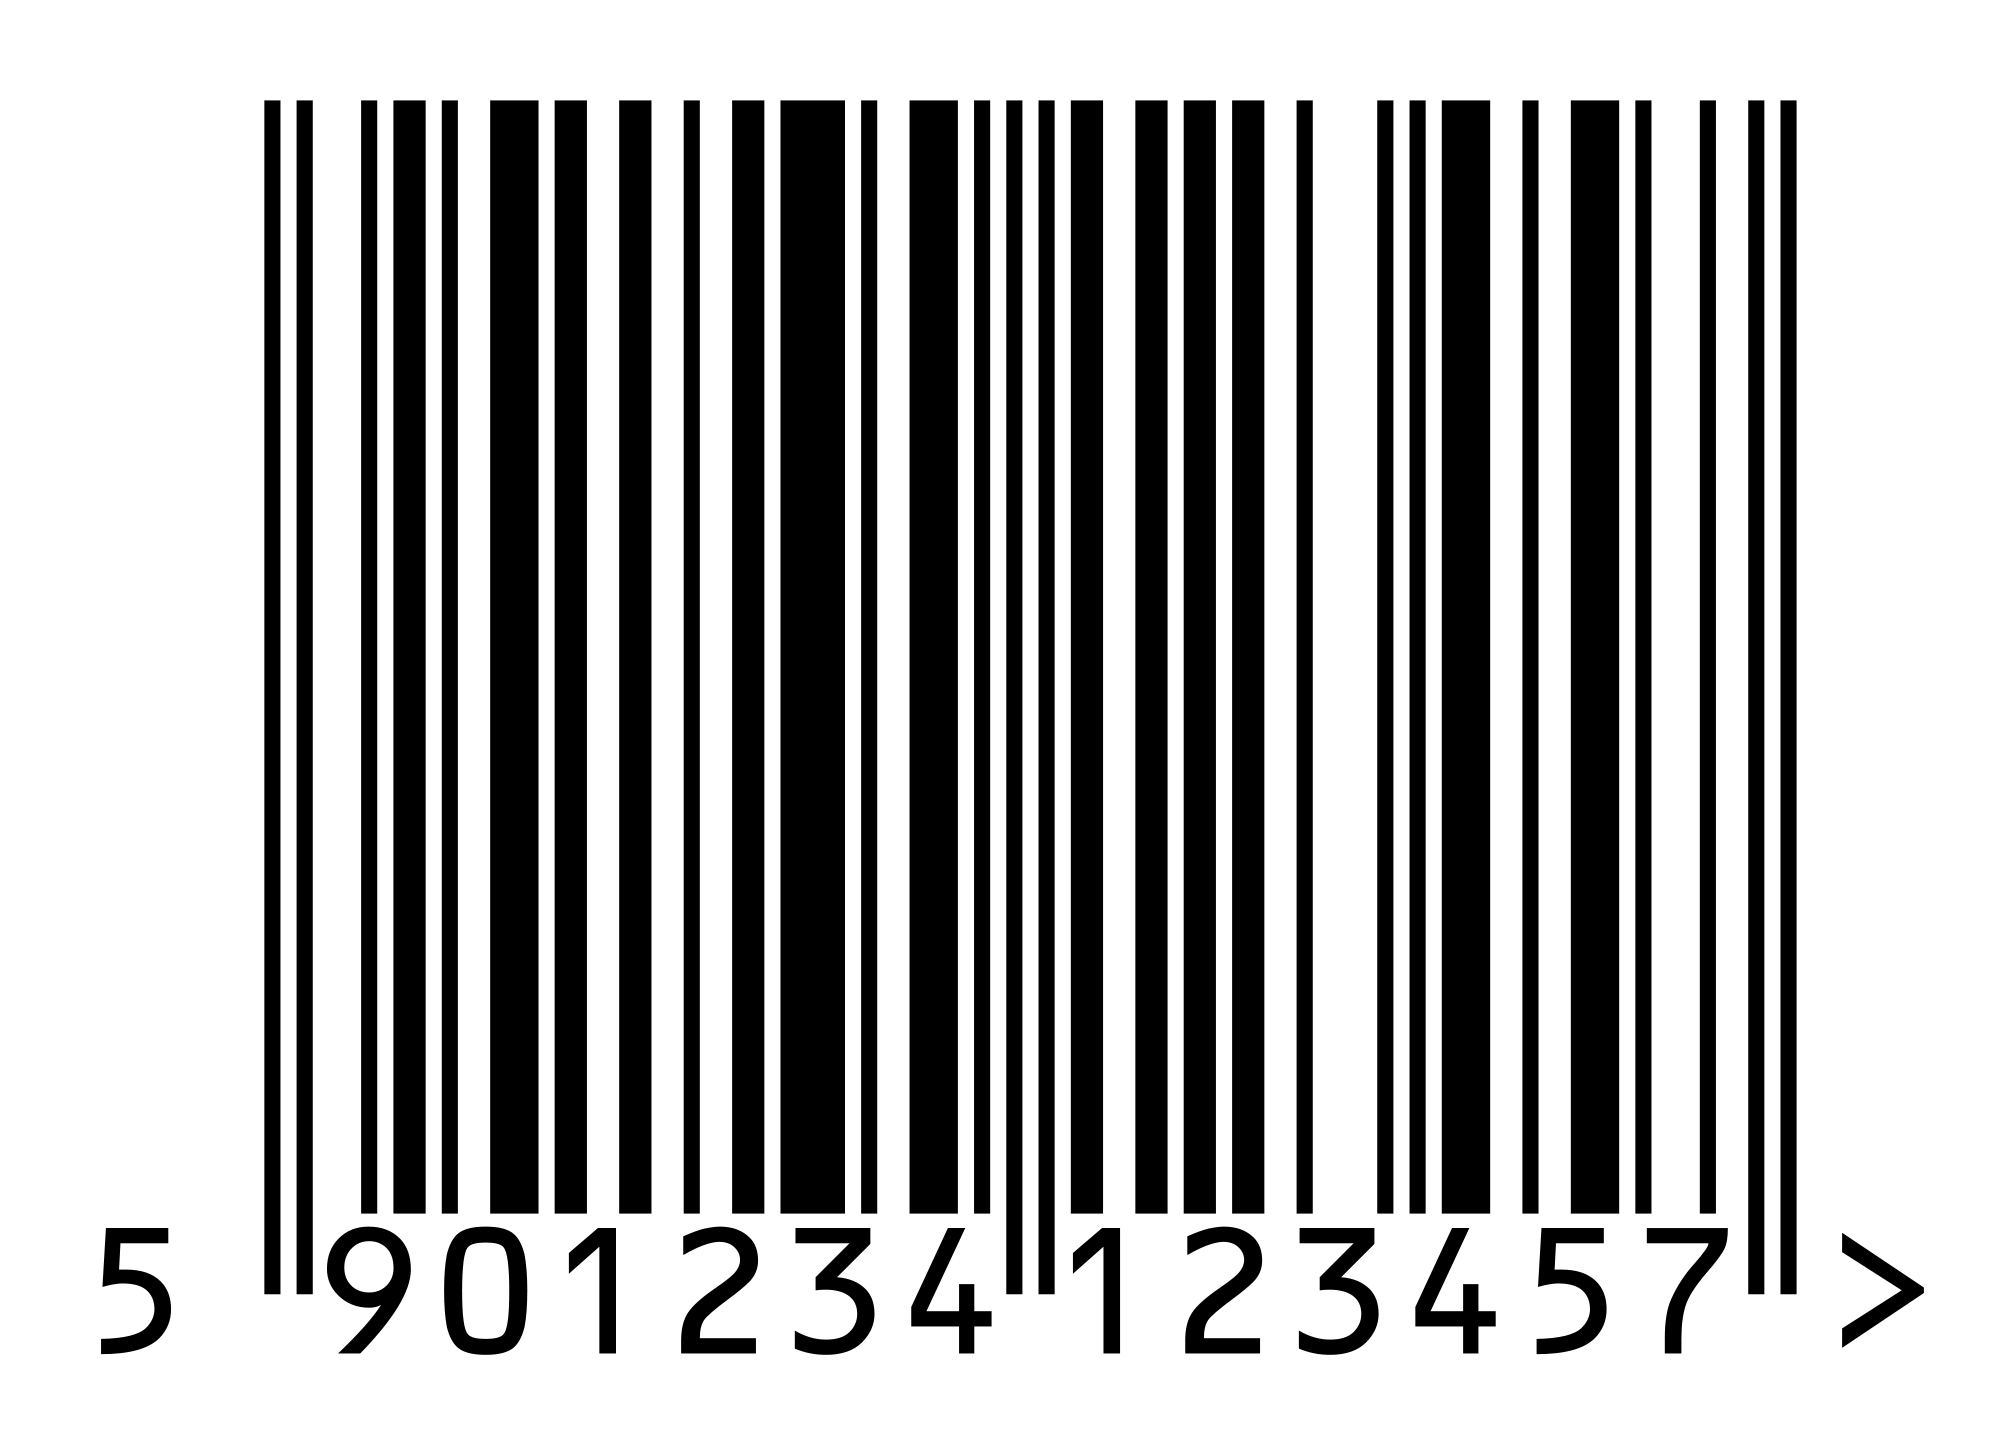
\includegraphics[width=0.25\textwidth]{Bilder/EAN_13.png}
	\vspace{-0.2cm}
	\caption[EAN-13 Strichcode]{EAN-13 Strichcode\footnotemark}
	\label{barcode}
\end{wrapfigure}
\footnotetext[1]{Quelle: \cite{Sakurambo2007}} 
%TODO
Für den Strichcode gibt es seit 1993 vier europäische Standards, die sich durch Einsatzgebiet (Handel/Industrie), Zeichenvorrat und Zeichensatz unterscheiden: ISO 15420 (EAN), ISO 15417 (Code 128), ISO 16388 (Code 39) und ISO 16390 (Code 2/5 Interleaved).
Der Strichcode wird vielfältig eingesetzt und heißt je nach Einsatzgebiet auch anders. Im Handel kennt man ihn unter der Bezeichnung EAN (European Article Number), in den Bereichen Materialfluss, Logistik und Lager als EAN128.

\subsection{Zweidimensionale Barcodes}
Zweidimensionale Barcodes enthalten Informationen entlang ihrer X- und ihrer Y-Achse. Anders gesagt, horizontal werden andere Daten codiert als vertikal.
Damit der Code richtig entschlüsselt werden kann, muss ein Scanner beide Dimensionen simultan, das Symbol also als Ganzes erfassen. Dies ist möglich durch verschieben der Scanlinie eines Laserscanners oder durch verwenden eines Laserscannerarrays welches als Kamera fungiert. Ebenso ist der Einsatz einer Kamera möglich, die den Code anschließend durch bildverarbeitende Algorithmen entschlüsselt.

\subsubsection{Stapelcode}
Stapelcodes bestehen aus mehreren Lagen von linearen Barcodes, die vertikal übereinander angeordnet wurden.
Der spezielle Typ 'Composite Bar Code' besteht aus einem linearen und einem zweidimensionalen Part.

\subsubsection{Matrixcodes}
Matrixcodes codieren Daten durch benutzen von Zellen innerhalb einer Matrix (daher auch der Name). Diese benutzten Zellen werden für die Darstellung innerhalb des Symbols schwarz gefärbt. Jede Zelle innerhalb des Codes ist gleich groß. 
Vorteile der Matrixcodes: Es werden viele Daten auf kleinem Raum gespeichert, die Lesbarkeit ist hoch, der Code kann auch bei schlechter Druckqualität oder Beschädigung noch gelesen werden und unterstützt den vollen ASCII Zeichensatz.
Nachteil: Es benötigt eher eine Kamera als einen Laserscanner, um den Code zu lesen. 
\samepage
\paragraph{QR-Code}~

\begin{wrapfigure}[7]{l}{0.35\textwidth}
	\centering
	\vspace{-0.65cm}
	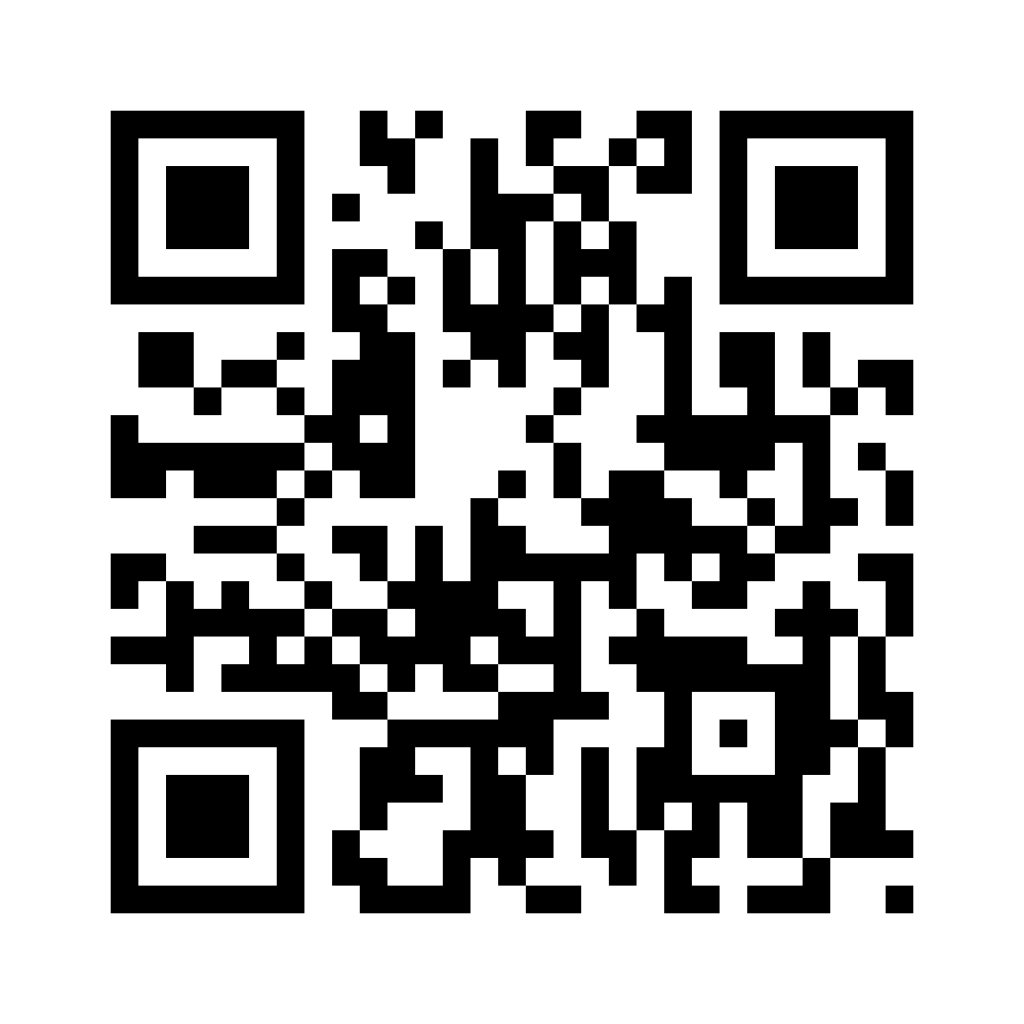
\includegraphics[width=0.2\textwidth]{Bilder/QR_Code.png}
	\vspace{-0.2cm}
    \caption[QR-Code]{QR-Code\footnotemark}
	\label{qrcode}	
\end{wrapfigure}
\footnotetext[2]{Quelle: \cite{brdall2009}}
Der QR-Code (ausgeschrieben \textit{Quick-Response}) wurde 1994 von der japanischen Firma Denso entwickelt. Heute wird er hauptsächlich in der Automobilindustrie und als Smartphone-Code verwendet; hier vor allem für Mobile Ticketing beziehungsweise Mobile Marketing. Diese mobile Anwendung ist auch auf seine hohe Fehlertoleranz zurückzuführen. Da der QR-Code den Hauptteil dieser Arbeit ausmachen soll, finden sich weiter Informationen und Details im entsprechenden Kapitel.

\paragraph{Data Matrix}


\subsection{Dreidimensionale Barcodes}
Es gibt zwei verschiedene Arten von Barcodes, die als 3D-Code bezeichnet werden:
Zum einen die fühlbaren Codes mit unterschiedlichen Erhebungen und zum anderen die Farbcodes oder auch "farbige QR-Codes", bei denen die Farbe die dritte Dimension darstellt.
~\pagebreak
